\chapter{Järjestelmän tietosisältö}
\section{Käsitekaavio}

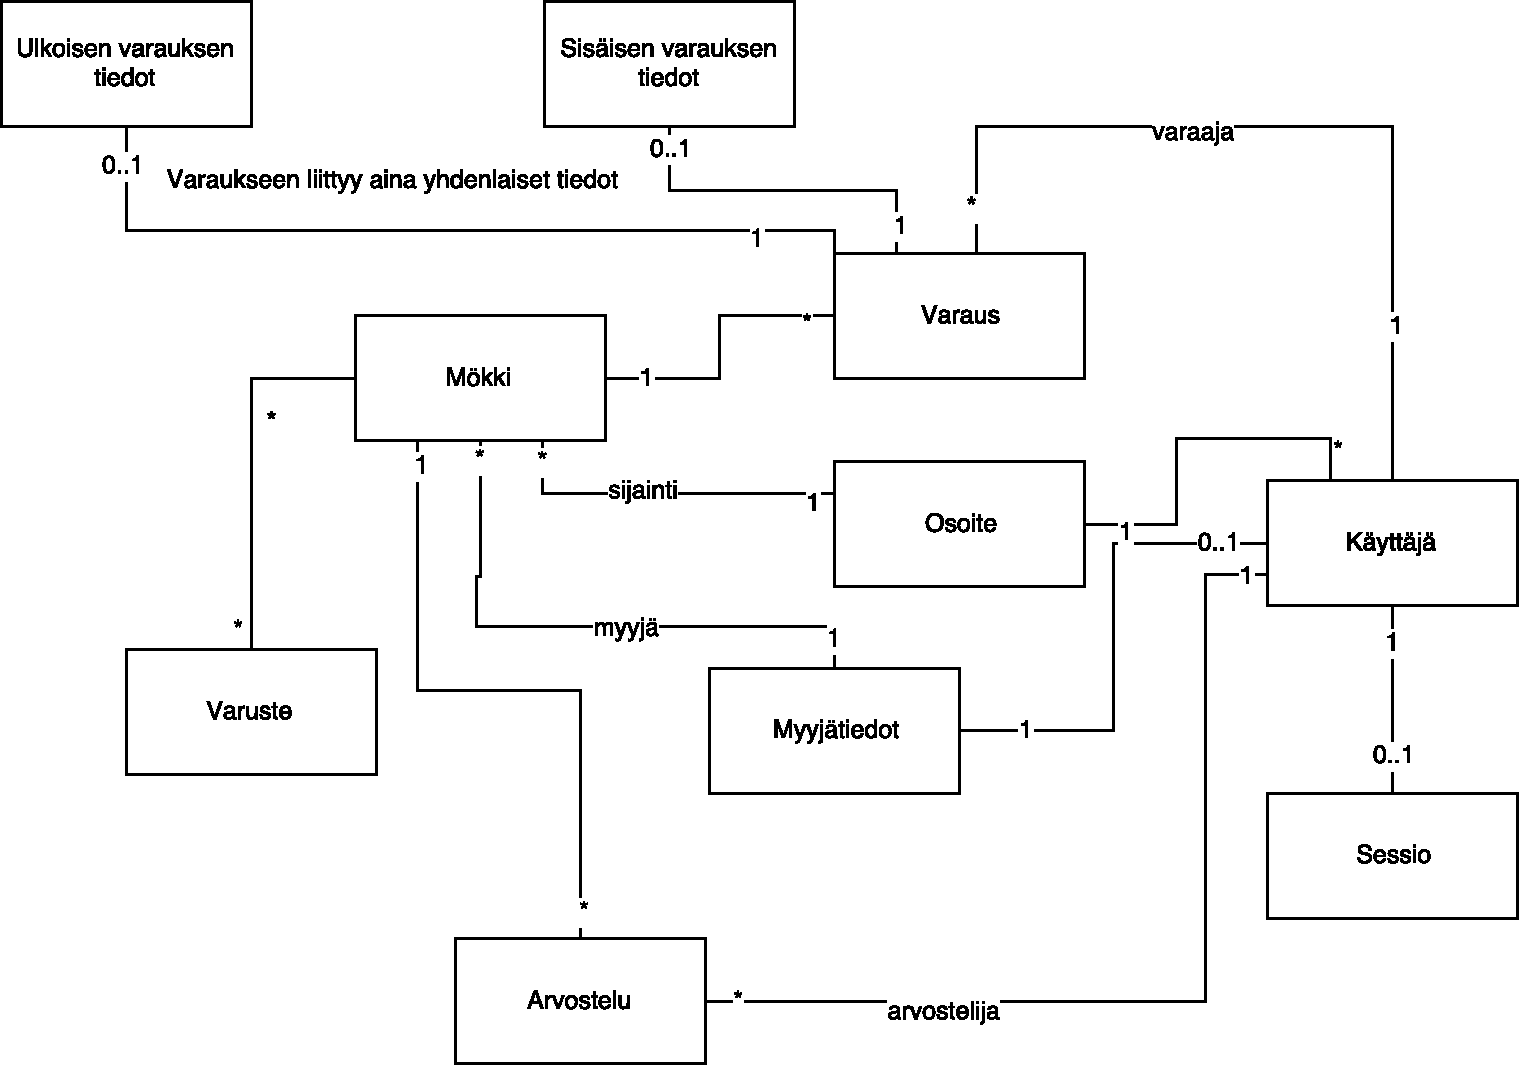
\includegraphics[width = 14cm]{./diagrams/drawio_entities.pdf}
\newpage
\section{Selitteet}

\subsection{Käyttäjä}
\begin{tabular}{|l|l|l|}
	\hline
	Attribuutti & Arvojoukko & Kuvaus \\ \hline
	Rooli & Yksi järjestelmän rooleista & \\ \hline
	Nimi & Rajoittamaton määrä tekstiä & Käyttäjän kutsumanimi. \\ \hline
	Sähköposti & 255 merkkiä tekstiä & \\ \hline
	Salasana & 60 merkkiä tekstiä & BCrypt-salasanatiiviste ja salt. \\ \hline
	Puhelin & Rajoittamaton määrä tekstiä & \\ \hline
	Osoiteviite & Validi viite osoitetauluun & Käyttäjän laskutusosoite. \\ \hline
\end{tabular}

\subsection{Myyjätiedot}
Lisätietoa käyttäjään, jos käyttäjä on vahvistettu ja hyväksytty myyjä.

\subsection{Varuste}
Mökin varuste tai myyntiargumentti \textit{("amenity")}.

\subsection{Varaus}
Tiedot varauksesta, johon kuuluu varatun mökin tunnus, varauksen kesto ja varaustyyppi. Varaukseen kuuluu aina tyypistä riippuen joko sisäisen tai ulkoisen varauksen lisätietoja.

\subsection{Sisäisen varauksen tiedot}
Lisätietoa varaukseen, jos varaus on tehty järjestelmän sisällä (= sivustolla). Sisältää varaajan käyttäjätunnuksen ja varauksesta maksetun hinnan.

\subsection{Ulkoisen varauksen tiedot}
Lisätietoa varaukseen, jos varaus on tehty järjestelmän ulkopuolella mökin omistajan toimesta (esimerkiksi oman varauksen tai remontin takia). Sisältää selitekentän.